\usetikzlibrary{arrows}
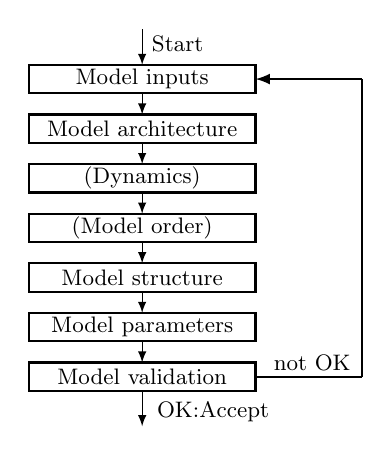
\begin{tikzpicture}[scale=0.9,transform shape]

\draw [thick] (-9.7,6.2) rectangle (-6.5,5.8);
\draw [thick] (-9.7,5.5) rectangle (-6.5,5.1);
\node at (-8.1,6) {\small Model inputs};

\node at (-8.1,5.3) {\small Model architecture};
\node at (-8.1,4.6) {\small (Dynamics)};
\node at (-8.1,3.9) {\small (Model order)};
\node at (-8.1,3.2) {\small Model structure};
\node at (-8.1,2.5) {\small Model parameters};
\node at (-8.1,1.8) {\small Model validation};
\node at (-7.6,6.5) {\small Start};
\node at (-7.1,1.3) {\small OK:Accept};
\node at (-5.7,2) {\small not OK};

\draw [thick][-latex] (-9.7,4.1) rectangle (-6.5,3.7);
\draw [thick][-latex] (-9.7,4.4) rectangle (-6.5,4.8);
\draw [thick][-latex] (-9.7,3.4) rectangle (-6.5,3);
\draw [thick][-latex] (-9.7,2.7) rectangle (-6.5,2.3);
\draw [thick][-latex] (-9.7,2) rectangle (-6.5,1.6);
\draw [-latex](-8.1,5.8) -- (-8.1,5.5);
\draw [-latex](-8.1,5.1) -- (-8.1,4.8);
\draw [-latex](-8.1,4.4) -- (-8.1,4.1);
\draw [-latex](-8.1,3.7) -- (-8.1,3.4);
\draw [-latex](-8.1,3) -- (-8.1,2.7);
\draw [-latex](-8.1,2.3) -- (-8.1,2);
\draw [-latex](-8.1,1.6) -- (-8.1,1.1);
\draw [-latex](-8.1,6.7) -- (-8.1,6.2);
\draw [thick](-5,6) -- (-5,1.8);


\draw [thick](-6.5,1.8) -- (-5,1.8);
\draw [thick][-latex](-5,6) -- (-6.5,6);
\end{tikzpicture}